\chapter{Planejamento do estudo de caso}
\label{cap_estudo_caso}

Neste capítulo descreveremos o planejamento realizado para a execução de um estudo de caso múltiplo.  Por meio dele, observaremos a adequação do modelo para a estimação dos juros em projetos reais hospedados em uma plataforma pública de versionamento de software. Descreveremos as etapas desse estudo de caso e quais ferramentas foram utilizadas para realizá-las.


\section{Introdução}

De acordo com Wohlin et al.\cite{wohlin2003empirical}, um estudo de caso é um método de pesquisa em que são utilizados dados de situações reais. Diferentemente de um experimento, no estudo de caso o pesquisador tem menos ou nenhum controle sobre os acontecimentos.  No contexto de projetos de software, um estudo de caso tem como objetivo monitorar as atividades realizadas durante o projeto. Segundo Yin, Robert K\cite{yin2011applications}, existem dois tipos de estudo de caso: os únicos e os múltiplos. Os estudos de casos únicos são aqueles em que os dados são obtidos de um único ``caso'',  que pode ser um projeto, uma empresa, um indivíduo ou qualquer outra unidade que seja apropriada para o estudo do objeto da pesquisa. Por outro lado, um estudo de caso múltiplo envolve diferentes unidades de interesse. Ou seja, são consideras diversas empresas, projetos, indivíduos, etc. A realização de casos múltiplos é mais indicada já que ela facilita generalização dos resultados obtidos por fornecerem múltiplas visões a respeito do objeto de pesquisa. Tendo isso em vista,  para avaliarmos o modelo de estimação do comportamento dos juros da dívida técnica descrito no capítulo \ref{estimacao:juros}, realizaremos um estudo de caso múltiplo envolvendo 1814 projetos armazenados em um repositório de software.

O objetivo deste estudo de caso será avaliar a consistência do modelo criado para estimar a dívida técnica em  projetos de software livre. Em outras palavras, vamos avaliar a aplicação de uma instância do modelo de estimação. Essa instância foi criada observando as particularidades dos projetos de software livre e também observando as limitação nos dados que temos disponíveis da plataforma GitHub.

\section{Dados do estudo de caso}


Conforme argumentado por Brown, N et al.\cite{brown2010managing}, há uma predominância na utilização de métodos qualitativos nas pesquisas a respeito da dívida técnica e isso pode levar a conclusões baseadas em intuições atraentes, porém não necessariamente corretas. Essas conclusões incorretas podem ser explicadas pela existência de dados obtidos por meio de declarações imprecisas. Essas declarações podem ser dadas pela dificuldade que as pessoas envolvidas com os projetos de software têm em assumir suas deficiências ou falhas. Por isso, Brown, N et al.\cite{brown2010managing} indicam a necessidade da criação de modelos baseados em abordagens quantitativas para viabilizar a criação de rigorosas técnicas de gerenciamento da dívida técnica que possam ser aplicadas em projetos de larga escala.

De acordo com Creswell\cite{w2016research}, uma pesquisa quantitativa tem como foco principal a quantificação de relacionamentos ou a comparação de um ou mais grupos. Adicionalmente, conforme explicado por Wohlin et al.\cite{wohlin2003empirical}, as pesquisas quantitativas são apropriadas quando existe a necessidade de testar o efeito de alguma atividade ou manipulação. Segundo Wang at al. \cite{wang201331}, a abordagem quantitativa disponibiliza uma série de ferramentas para descobrir, com um determinado nível de confiança, a verdade a respeito de um objeto de estudo. O que diferencia, substancialmente, uma pesquisa quantitativa de outra qualitativa, é seu grau de  objetividade a respeito dos fenômenos avaliados. Na abordagem quantitativa há pouco ou nenhuma margem para que haja, durante o processo de coleta de dados, uma interpretação dos indivíduos relacionados com o evento analisado. Ao invés disso, são utilizados apenas fatos que não dependem de sensações, reflexões, intuições ou qualquer outra forma subjetiva de avaliação. Isso faz com que os dados numéricos sejam predominantes em pesquisas quantitativas.  Essa característica permite que, utilizando poucos recursos, um grande volume de dados possa ser coletado e analisado.  Amaratunga et al. \cite{amaratunga2002quantitative} lista algumas das principais características de uma pesquisa quantitativa:

\begin{itemize}
\item Permitem a replicação e a comparação de resultados.
\item Assegura a independência entre o observador e o objeto observado.
\item Proporciona maior objetividade para a determinação da confiabilidade e a validade dos resultados.
\item Enfatiza a necessidade de formular hipóteses para subsequentes verificações.
\end{itemize}



Por essas razões, obtemos os dados utilizados neste estudo de caso por meio de técnicas quantitativas oriundas da área de mineração de repositórios.

\subsection{Mineração de repositórios}

Plataformas como GitHub, SourceForge e Bitbucket ganharam popularidade devido à evolução nas ferramentas de controle de versão e ao reconhecimento, por parte da comunidade de software,  das vantagens de utilizarem-se ferramentas de colaboração. Além de ferramentas para armazenamento e organização do código, essas plataformas fornecem uma variedade de facilidades para a interação entre os colaboradores dos projetos. Com isso, essas ferramentas acumularam uma quantidade imensa de dados sobre os projetos hospedados e a forma como colaboradores interagem com esses projetos. Esses dados têm sido reconhecidos como altamente relevantes para as pesquisas quantitativas na área de engenharia de software. Foi chamado de mineração de repositórios de software \cite{bai2008mining} o conjunto de técnicas de investigação que utilizam informações provenientes de repositórios de software. Como exemplos de estudos que exploram essas técnicas, podemos citar aqueles envolvendo a predição de defeitos \cite{wang2014software}, propagação de mudanças \cite{wiese2015predicting} e confiabilidade do software \cite{de2015software}. Neste trabalho, utilizaremos a mineração de repositórios de software para extrairmos os dados para o estudo de caso. 


\section{Etapas do estudo de caso}

O estudo de caso será realizado em cinco etapas conforme ilustrado na Figura \ref{fig:cap_metodo_resumo_etapas}.  






  \begin{figure}[H]
  \centering
  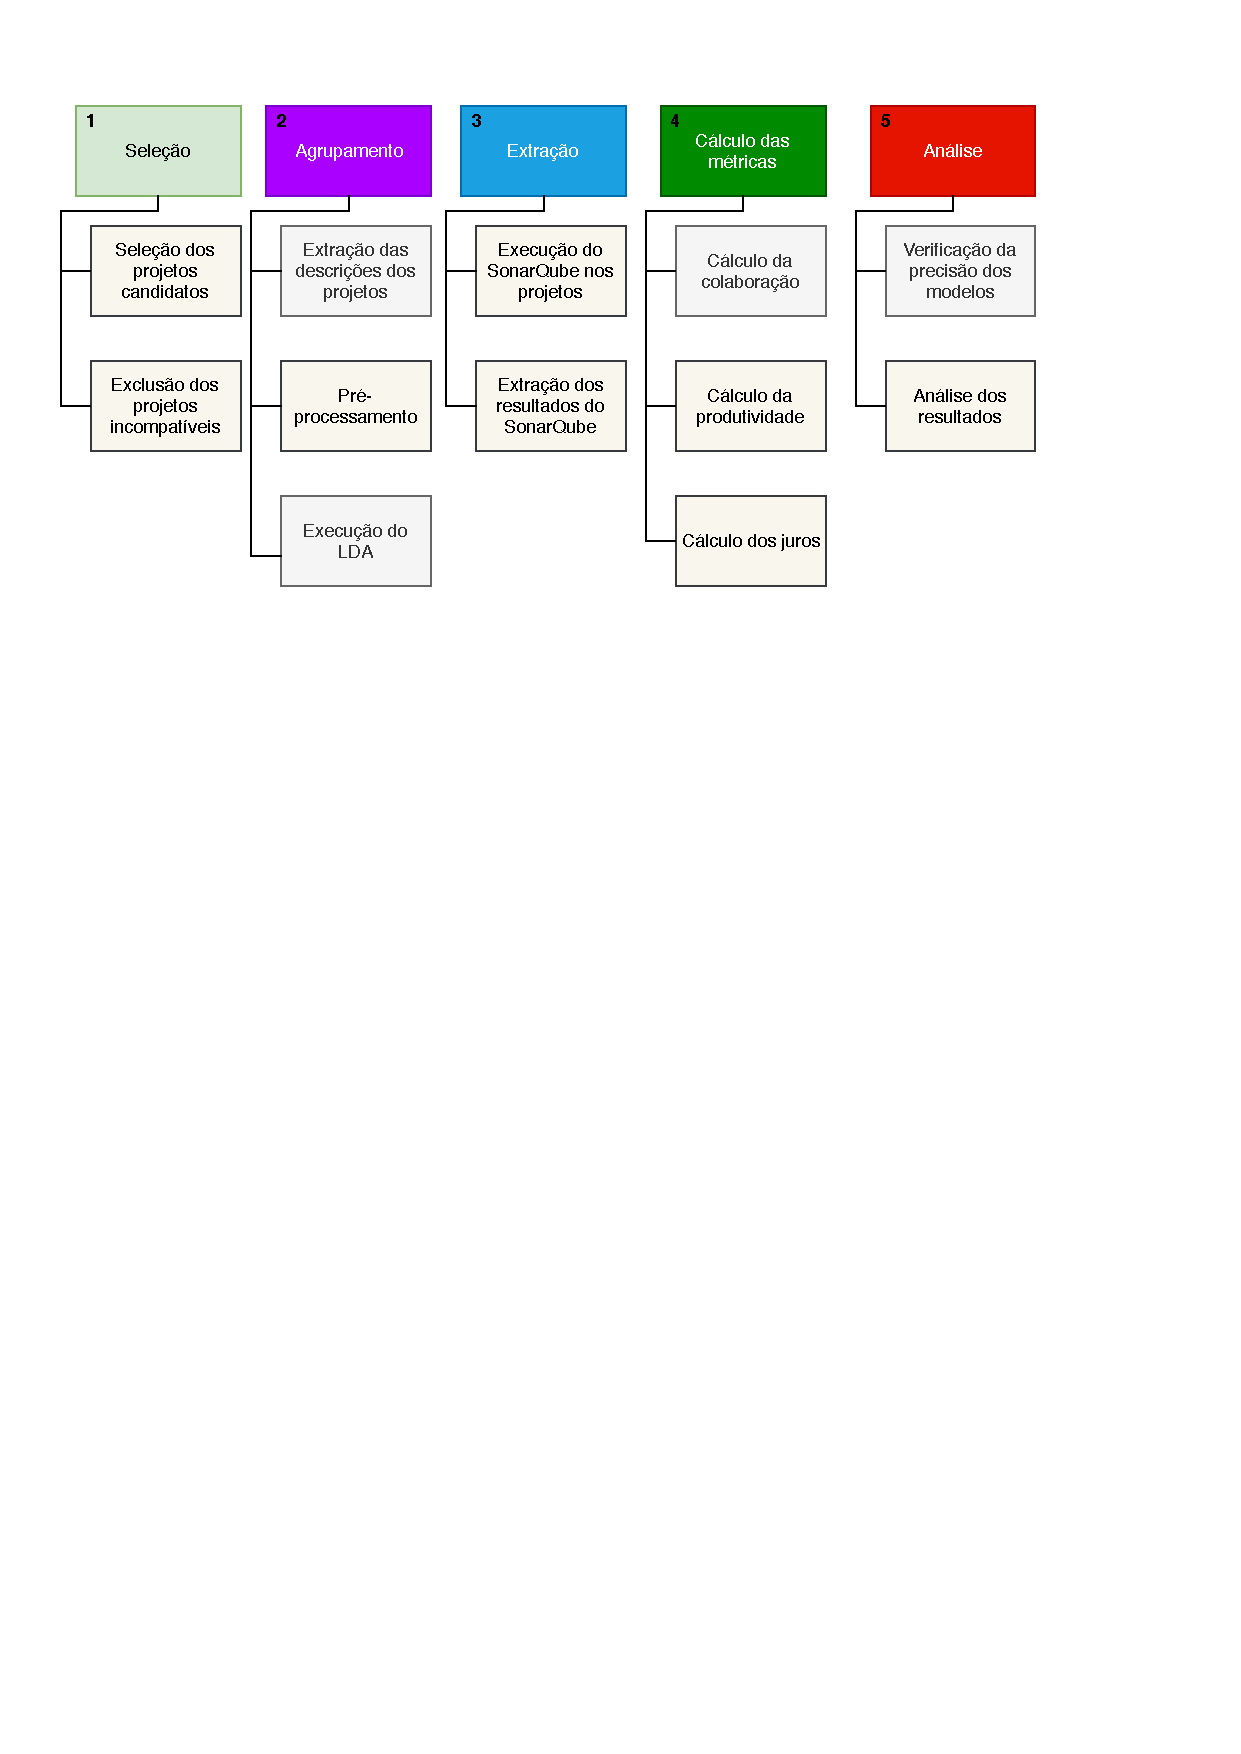
\includegraphics[trim={0.4cm 19.5cm 0cm 1cm},clip]{capitulo_metodo/ResumoEtapas.pdf} 
  \caption{Resumo das etapas do estudo de caso. }
  \label{fig:cap_metodo_resumo_etapas} 
\end{figure}

A seguir forneceremos um breve resumo a respeito das etapas e atividades do estudo de caso:

\begin{enumerate}
\item \textbf{Seleção}: Criação de uma lista com todos os projetos que serão analisados no estudo de caso.
   \begin{enumerate}
      \item \textit{Seleção dos projetos candidatos}: Inclusão de todos os projetos que atendam a alguns critérios básicos como a linguagem de programação utilizada.
      \item \textit{Exclusão dos projetos incompatíveis}: Remoção de projetos por meio de heurísticas criadas para evitar a análise de repositórios que, na verdade, não são projetos de software ou que não possam ser analisados por algum impedimento operacional.
   \end{enumerate}
\item \textbf{Agrupamento}: Criação de grupos de projetos que sejam de um mesmo domínio de aplicação como gerenciadores de banco de dados, sistemas operacionais, jogos e bibliotecas. O agrupamento será realizado por meio de uma técnica de processamento de linguagem natural chamada \textit{Latent Dirichlet allocation}(LDA)\cite{blei2002latent}.
   \begin{enumerate}
      \item \textit{Extração das descrições dos projetos}: É necessário localizar e extrair a descrição do projeto para que ela possa ser utilizada no LDA.
      \item \textit{Pré-processamento}: São realizadas as diversas manipulações necessárias para que o LDA possa ser aplicado.
      \item \textit{Execução do LDA}: O algoritmo do LDA é executado na descrição pré-processada de cada projeto.
   \end{enumerate}
\item \textbf{Extração}: Aplicação da ferramenta SonarQube\cite{campbell2013sonarqube} para extração de diversas métricas comuns dos projetos.
  \begin{enumerate}
      \item \textit{Execução do SonarQube nos projetos}: A ferramenta é efetivamente executada para analisar o código-fonte de cada um dos projetos da pesquisa.
      \item \textit{Extração dos resultados do SonarQube}: As métricas relevantes para o estudo de caso são obtidas do resultado da aplicação do SonarQube.
   \end{enumerate}
\item \textbf{Cálculo das métricas}: Cálculo das métricas específicas do estudo de caso.
 \begin{enumerate}
      \item \textit{Cálculo da colaboração}: Aplicação de modelos para quantificar o volume e qualidade da colaboração de cada um dos projetos analisados.
      \item \textit{Cálculo da produtividade}: Aplicação do modelo de produtividade descrito na sessão \ref{modelo_de_estimacao_produtividade}.
       \item \textit{Cálculo dos juros}: Cálculo de uma estimativa dos juros da dívida técnica para os projetos.
   \end{enumerate}
\item \textbf{Análise}
\begin{enumerate}
      \item \textit{Verificação da precisão dos modelos}: Realização de uma breve análise estatística dos modelos de produtividade e colaboração.
      \item \textit{Análise dos resultados}: Discussão e análise dos resultados obtidos.
   \end{enumerate}
\end{enumerate}


\section{Ferramenta de automatização do estudo de caso: GitResearch}
\label{cap_estudo_caso_ferramenta}


Para automatizar uma parte das atividades realizadas neste estudo de caso foi construída uma ferramenta chamada GitResearch. Essa ferramenta foi desenvolvida na linguagem Java e está disponível em https://github.com/Jandisson/git-research. Ela foi desenvolvida por duas razões: facilitar a manipulação de uma grande quantidade de projetos em um tempo pequeno e permitir que os resultados obtidos nesta pesquisa possam ser reproduzidos mais facilmente. Apesar de ter sido desenvolvida especificamente para esta pesquisa, ela foi planejada de forma que possa ser utilizada, com as devidas alterações, em outras pesquisas que envolvam a extração e o  processamento de dados de repositórios de software como o GitHub.

Um dos requisitos almejados, durante a concepção do GitResearch, foi a possibilidade de processar uma grande quantidade de dados utilizando de forma satisfatória o hardware disponível. Isso foi alcançado ao realizar esse processamento de uma forma paralela. Ou seja, a ferramenta foi planejada de forma que as atividades em cada etapa da pesquisa pudessem ser realizadas em diversas linhas de execução. Além disso, houve a preocupação em criar uma arquitetura flexível que facilitasse a alteração das funcionalidades existentes e adição de novas funcionalidades. Para alcançar todos esses objetivos, escolhemos, como a base para o GitResearch, o framework Spring Batch\cite{cogoluegnes2011spring}. Utilizando esse framework vamos executar a tarefa de extração e processamento dos dados como um processo batch. De acordo com Martin. et al. \cite{martin2015batch}, um processamento batch acontece quando casos semelhantes são processados simultaneamente sem a intervenção de um usuário. Escolhemos esse modelo de processamento pois ele se adequa as nossas necessidades de desempenho e condiz com as tarefas que serão realizadas no estudo de caso.






\subsection{Arquitetura}

O GitResearch é baseado na arquitetura do Spring Batch. Um resumo dessa arquitetura é apresentado na Figura \ref{fig:arquitetura_gitresearch}. Um \textit{Job} representa um processo batch. Cada \textit{Job} possui um conjunto, que pode ser ou não ordenado, de \textit{Steps} que por sua vez são as atividades que devem ser realizadas durante o processamento. Tanto um \textit{Job} quanto um \textit{Step} utilizam um repositório de dados chamado de \textit{JobRepository}. Esse repositório armazena, principalmente, dados de controle a respeito de cada execução de um  \textit{Job}. Além disso, o repositório pode ser usado pelos \textit{Steps} para armazenar quaisquer informações que sejam necessárias para realizar o processamento. Cada \textit{Step} é formado por três objetos: \textit{ItemReader}, \textit{ItemProcessor}, \textit{ItemWriter}. Esses três objetos são responsáveis respectivamente por ler, processar e armazenar cada item do processo batch. Cada item será um dos projetos a serem processados neste estudo de caso. 


 \begin{figure}[H]
  \centering
  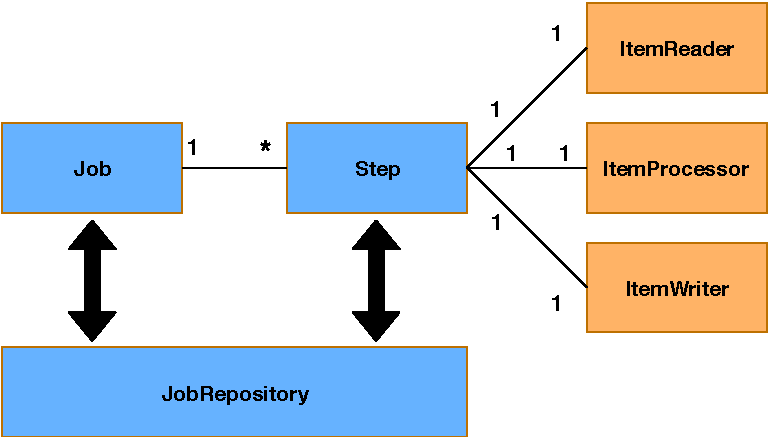
\includegraphics{capitulo_estudo_caso/springbatch_architecture.pdf} 
  \caption{Arquitetura do framework Spring Batch. Adaptada de \cite{minella2011pro}.}
  \label{fig:arquitetura_gitresearch} 
\end{figure}

Os passos realizados para criar o GitResearch, tendo como base o SpringBatch, foram os seguintes:


\begin{enumerate}
\item \textbf{Configuração do JobRepository}. Pode ser usado qualquer banco de dados que tenha suporte ao JDBC\cite{reese2000database}. Em nosso estudo de caso, utilizamos um banco de dados de código livre chamado Derby\cite{mei2010research}.  Ele foi escolhido por ser de fácil configuração e não requerer instalação. O banco de dados e gerenciador do banco de dados são armazenados em um único arquivo. Essa ação facilitará a reprodução do estudo de caso e, consequentemente, a validação dos resultados obtidos.
\item \textbf{Criação e configuração do \textit{Job}}. A configuração de um \textit{Job} consiste em indicar quais \textit{Steps} serão executadas e como essa execução deve ser feita. Nesse ponto é possível determinar qual será o fluxo de \textit{Steps}, a existência ou não paralelismos  e a quantidade de recursos, como linhas de execução, que deverá ser utilizada. A Figura \ref{fig:configuracao_job} apresenta o código de configuração do \textit{Job} no GitResearch. Em nosso caso, foi necessária apenas a configuração de um \textit{Job}.
\item \textbf{Implementação  dos  \textit{Steps} necessários}. Essa implementação consiste na criação dos \textit{ItemReader}, \textit{ItemProcessor} e \textit{ItemWriter}. Para um determinado \textit{Step}, é possível que não seja necessário criar novos \textit{ItemReader} ou \textit{ItemWriter}. Ao invés disso, é possível utilizar algum objeto previamente criado e disponibilizado pelo framework. Foi isso que foi realizado no GitResearch. A maioria dos \textit{Steps} utiliza algum \textit{ItemReader} ou \textit{ItemWriter} padrão do framework. Entretanto, no caso do \textit{ItemProcessor} não há como utilizar um objeto padrão já que esse elemento é o responsável pela lógica de processamento e isso é particular para cada aplicação. Com isso, a implementação dos \textit{Steps} já existentes no GitResearch como a implementação de novos \textit{Steps}, irá sempre exigir a escrita de novos \textit{ItemProcessor}. No GitResearch foi necessária a implementação de oito \textit{Steps} conforme ilustrado na Figura \ref{fig:passos_gitresearch}.  Conforme mostrado na Figura, a entrada para o processamento realizado pelo GitResearch é uma lista com todos os projetos que serão analisados. Ou seja, essa seleção dos projetos é uma atividade que não é realizada pelo GitResearch. Essa etapa será descrita no item \ref{secao_cap_estudo_selecao_projetos}.
\end{enumerate}



 \begin{figure}[H]
  \centering
   \frame{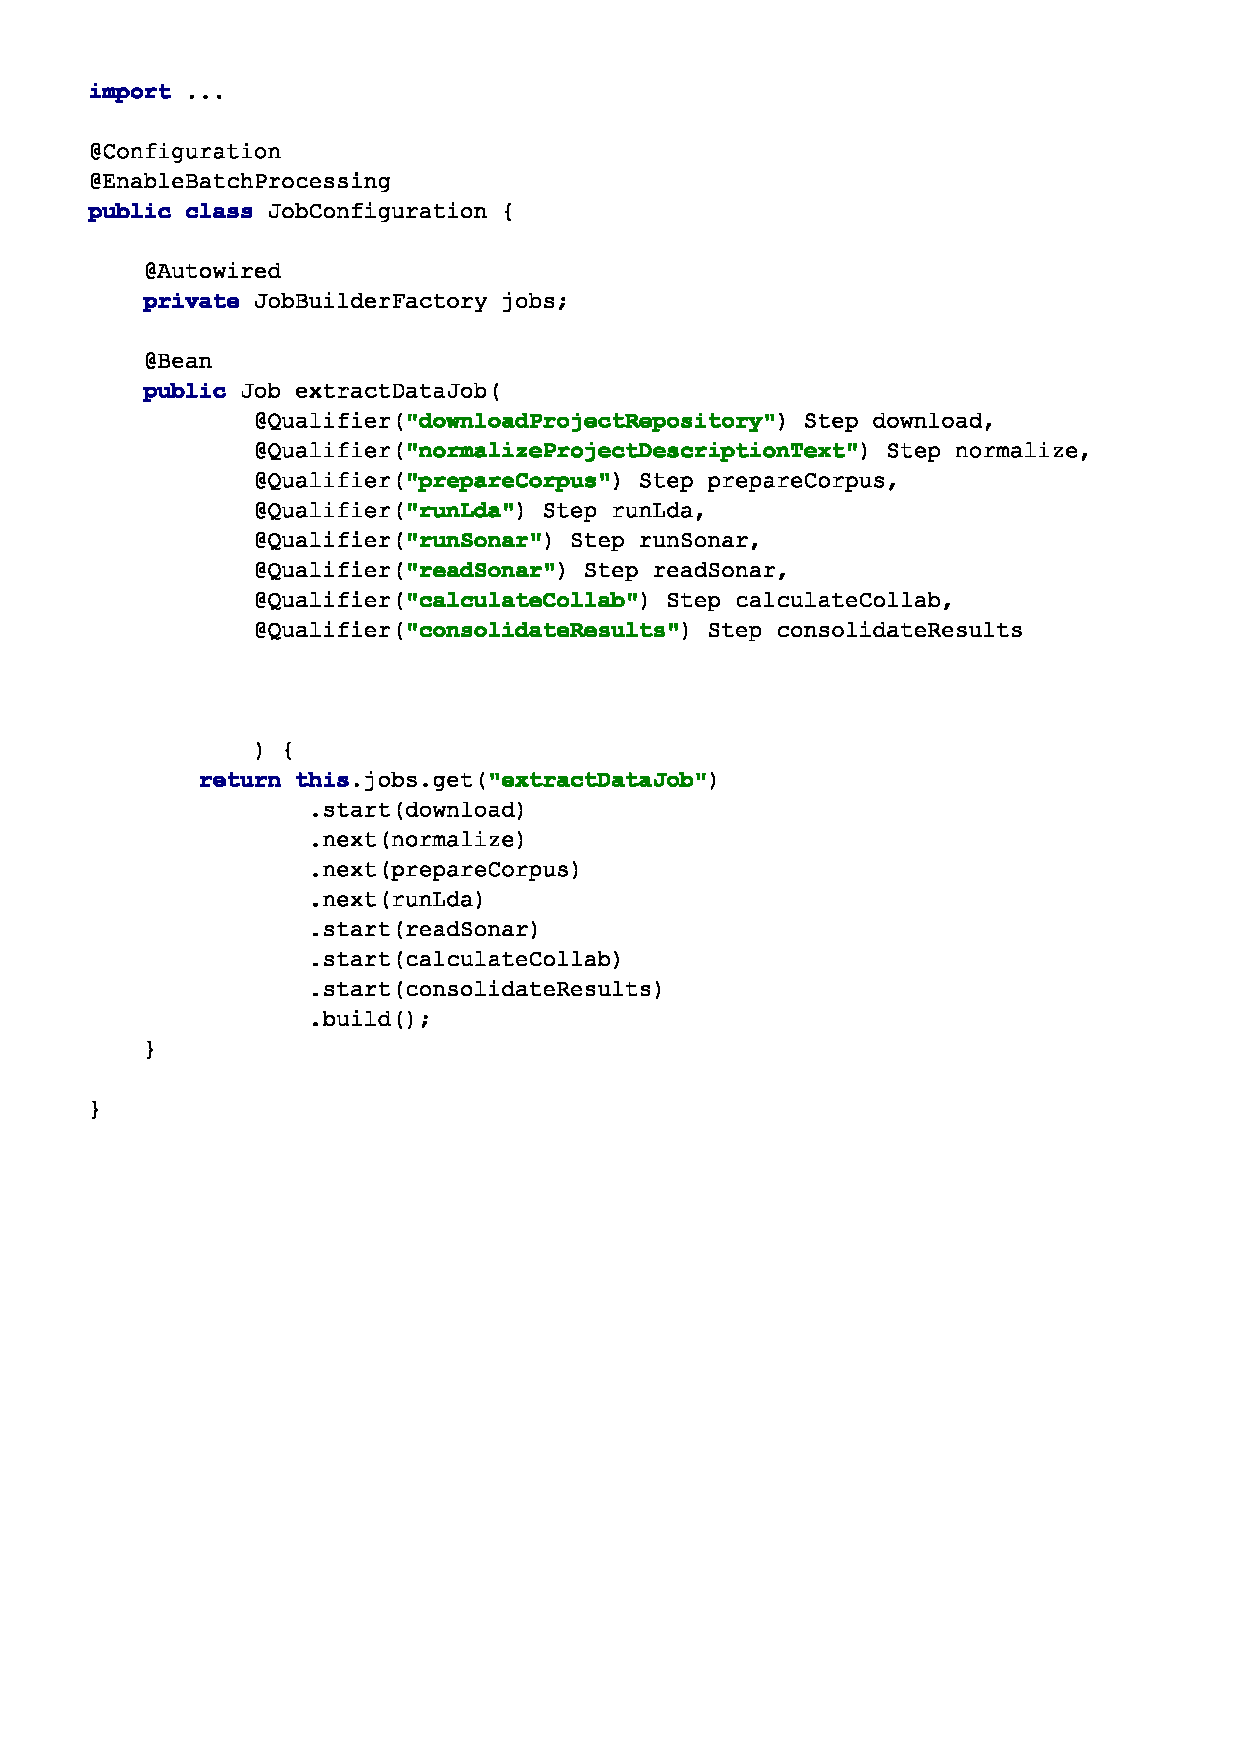
\includegraphics[trim={1cm 10cm 2.5cm 0},clip]{capitulo_estudo_caso/configuracao_job.pdf}} 
  \caption{Código responsável por configurar o \textit{Job} no GitResearch.}
  \label{fig:configuracao_job} 
\end{figure}
 
 
 \subsection{Passos do processamento}
 
 A Figura\ref{fig:passos_gitresearch} apresenta os passos de processamento no GitResearch.  Todas as etapas do estudo de caso descritas na Figura \ref{fig:cap_metodo_resumo_etapas} serão automatizadas ou semiautomatizadas por meio do GitResearch. A única exceção é a etapa de seleção dos projetos candidatos. Essa etapa inclui a aplicação de um série de heurísticas criadas com o intúito de excluir repositórios que não são projetos de software. A implementação dessas heurísticas demandaria uma quantidade significativa de tempo e poderia fazer com que o escopo da pesquisa fosse ultrapassado. Por isso, essa etapa de seleção foi realizada de uma forma semiautomática por meio de pesquisas no banco de dados de projetos.  Contudo, todos os procedimentos realizados foram devidamente documentados e serão apresentados na sessão \ref{secao_cap_estudo_selecao_projetos}.
 
Comparando a Figura \ref{fig:passos_gitresearch} e a Figura \ref{fig:cap_metodo_resumo_etapas}, podemos ver que há diferenças entre o de processamento do GitResearch e as etapas do estudo de caso. Essa distinção aconteceu porque houve a necessidade da criação de passos de processamento que não estavam explícitos nas etapas do estudo de caso. Um exemplo é o passo de processamento ``Download dos projetos''. Outra razão da diferença é a necessidade de agrupar ou separar alguns passos de processamento no GitResearch por uma questão de desempenho.  Na Figura \ref{fig:cap_metodo_mapeamento_estudo_gitresearch} apresentamos um mapeamento entre as etapas do estudo de caso e os passos de processamento no GitResearch. 

 \begin{figure}[H]
  \centering
  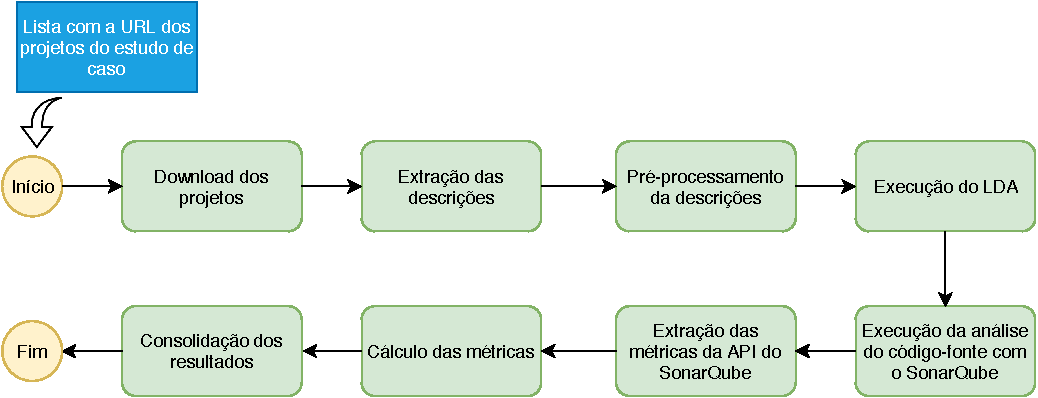
\includegraphics{capitulo_estudo_caso/git_research_steps.pdf} 
  \caption{Passos do processamento no GitResearch.}
  \label{fig:passos_gitresearch} 
\end{figure}




  \begin{figure}[H]
  \centering
  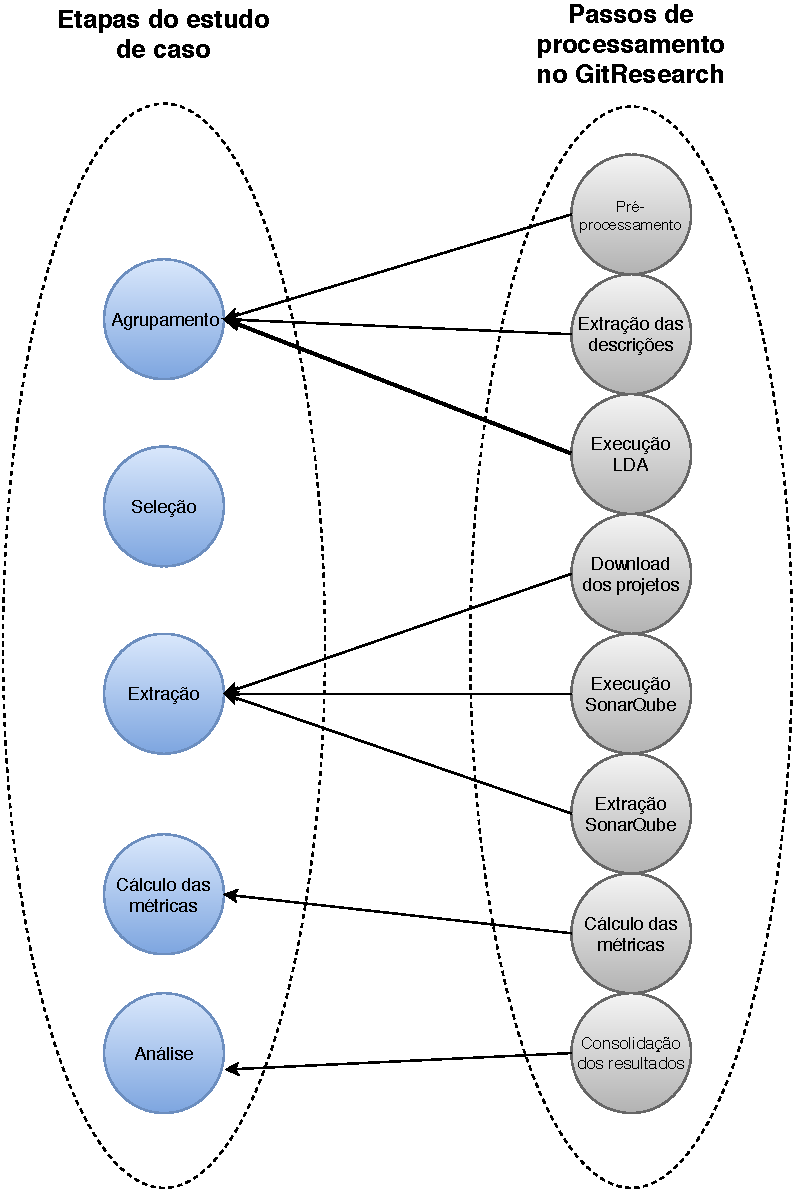
\includegraphics{capitulo_estudo_caso/mapeamento_etapas_estudo_gitresearch.pdf} 
  \caption{Mapeamento entre as etapas do estudo de caso e as etapas de processamento no GitResearch. }
  \label{fig:cap_metodo_mapeamento_estudo_gitresearch} 
\end{figure}
 





\section{Outras ferramentas utilizadas}

Para a execução dos estudo de caso foram necessárias, além do GitResearch, outras ferramentas e plataformas já existentes. Nesta sessão descreveremos essas ferramentas e como elas foram utilizadas neste estudo de caso.


\subsection{GitHub}
\label{cap_estudo_github}

No contexto do \textit{open source}, tornar público o código-fonte de um projeto de software não se trata apenas de uma característica positiva; na verdade, essa tendência é uma necessidade que caracteriza os princípios dessa filosofia de desenvolvimento de software. A comunidade interessada no software deve ter livre acesso a ele para que possa usá-lo, alterá-lo e distribuí-lo. Por conta dessas necessidades, houve uma popularização dos repositórios públicos de software. Esse tipo de plataforma fornece aos usuários meios para acessar o código  de terceiros como também permite que eles mesmos disponibilizem seus projetos de software. A popularização dessas plataformas fez com que elas fossem a fonte de uma grande quantidade de dados. Esses dados são produzidos de diversas formas, seja pela extração a partir do código-fonte seja pela interação realizada entre os usuários.  Em todos os casos, a facilidade de acesso e a pluralidade de dados fazem com que os repositórios de software sejam uma opção interessante para a obtenção de dados para pesquisas. Em nosso estudo de caso, obteremos dados do GitHub: um repositório de projetos  de software baseado na tecnologia versionamento Git\cite{loeliger2012version}. No Apêndice \ref{apendice_git} apresentamos maiores informações a respeito do protocolo Git. 


O GitHub é uma plataforma online para o armazenamento de repositórios. O que diferencia o GitHub de um servidor Git convencional é o conjunto de funcionalidades adicionais que a plataforma disponibiliza aos seus usuários. Essas funcionalidades não só são adições aos recursos de versionamento que o Git já disponibiliza como também são recursos sociais que permitem a interação entre os usuários. De acordo com  Dabbish et al. \cite{dabbish2012social} essas funcionalidades socias facilitam a colaboração entre os usuários pois viabilizam que eles monitorem as atividades de uma grande quantidade de projetos além de gerar uma grande quantidade de dados. Esses dados, publicamente disponíveis,  têm sido usados ativamente como uma fonte para pesquisas científicas. 






\subsection{GHTorrent}

O GitHub disponibiliza seus dados por meio de uma API. Nessa API é possível não apenas pesquisar informações a respeito de um repositório específico como também buscar repositórios utilizando critérios como linguagem, data de criação e descrição. Porém, devido a questões de segurança, essa API impõe severas restrições de acesso aos seus usuários.  Existe uma quantidade pequena de requisições que podem ser realizadas por hora. Além disso, é necessário um esforço de desenvolvimento para que os dados obtidos possam ser armazenados e principalmente relacionados entre si. Devido a essas dificuldades, surgiram projetos como o GHTorrent, um banco de dados  criado por Gousious et al. \cite{gousios2012ghtorrent} que espelha as informações contidas no GitHub. Esse projeto surgiu para distribuir de uma forma simples e rápida as informações disponibilizadas pela API do GitHub. Pesquisadores podem utilizar os dados no GitHub prontamente sem a necessidade de desenvolver um sistema que extraia e relacione esses dados.

O GHtorrent disponibiliza os dados por meio de arquivos de backup do banco e por meio de um banco de dados online onde os usuários podem se cadastrar e realizar consultas. Escolhemos obter os dados por meio do download de um arquivo de backup. Optamos por essa forma de acesso, pois queremos incluir uma grande quantidade de projetos em nosso estudo de caso. Por isso, teremos a necessidade de realizar a extração de dados com rapidez. Ao utilizar um backup completo do GHTorrent, pudemos importá-lo em um ambiente no qual o poder de processamento fosse compatível com nossas expectativas de desempenho.  O arquivo que utilizamos pode ser obtido no seguinte endereço: http://ghtorrent-downloads.ewi.tudelft.nl/mysql/mysql-2017-12-01.tar.gz. Esse arquivo contém os dados obtidos até o último dia de dezembro de 2017. A Figura \ref{fig:tabelas_ghtorrent} contém uma lista com as  principais tabelas encontrados no arquivo do GHTorrent.


 \begin{figure}[H]
  \centering
  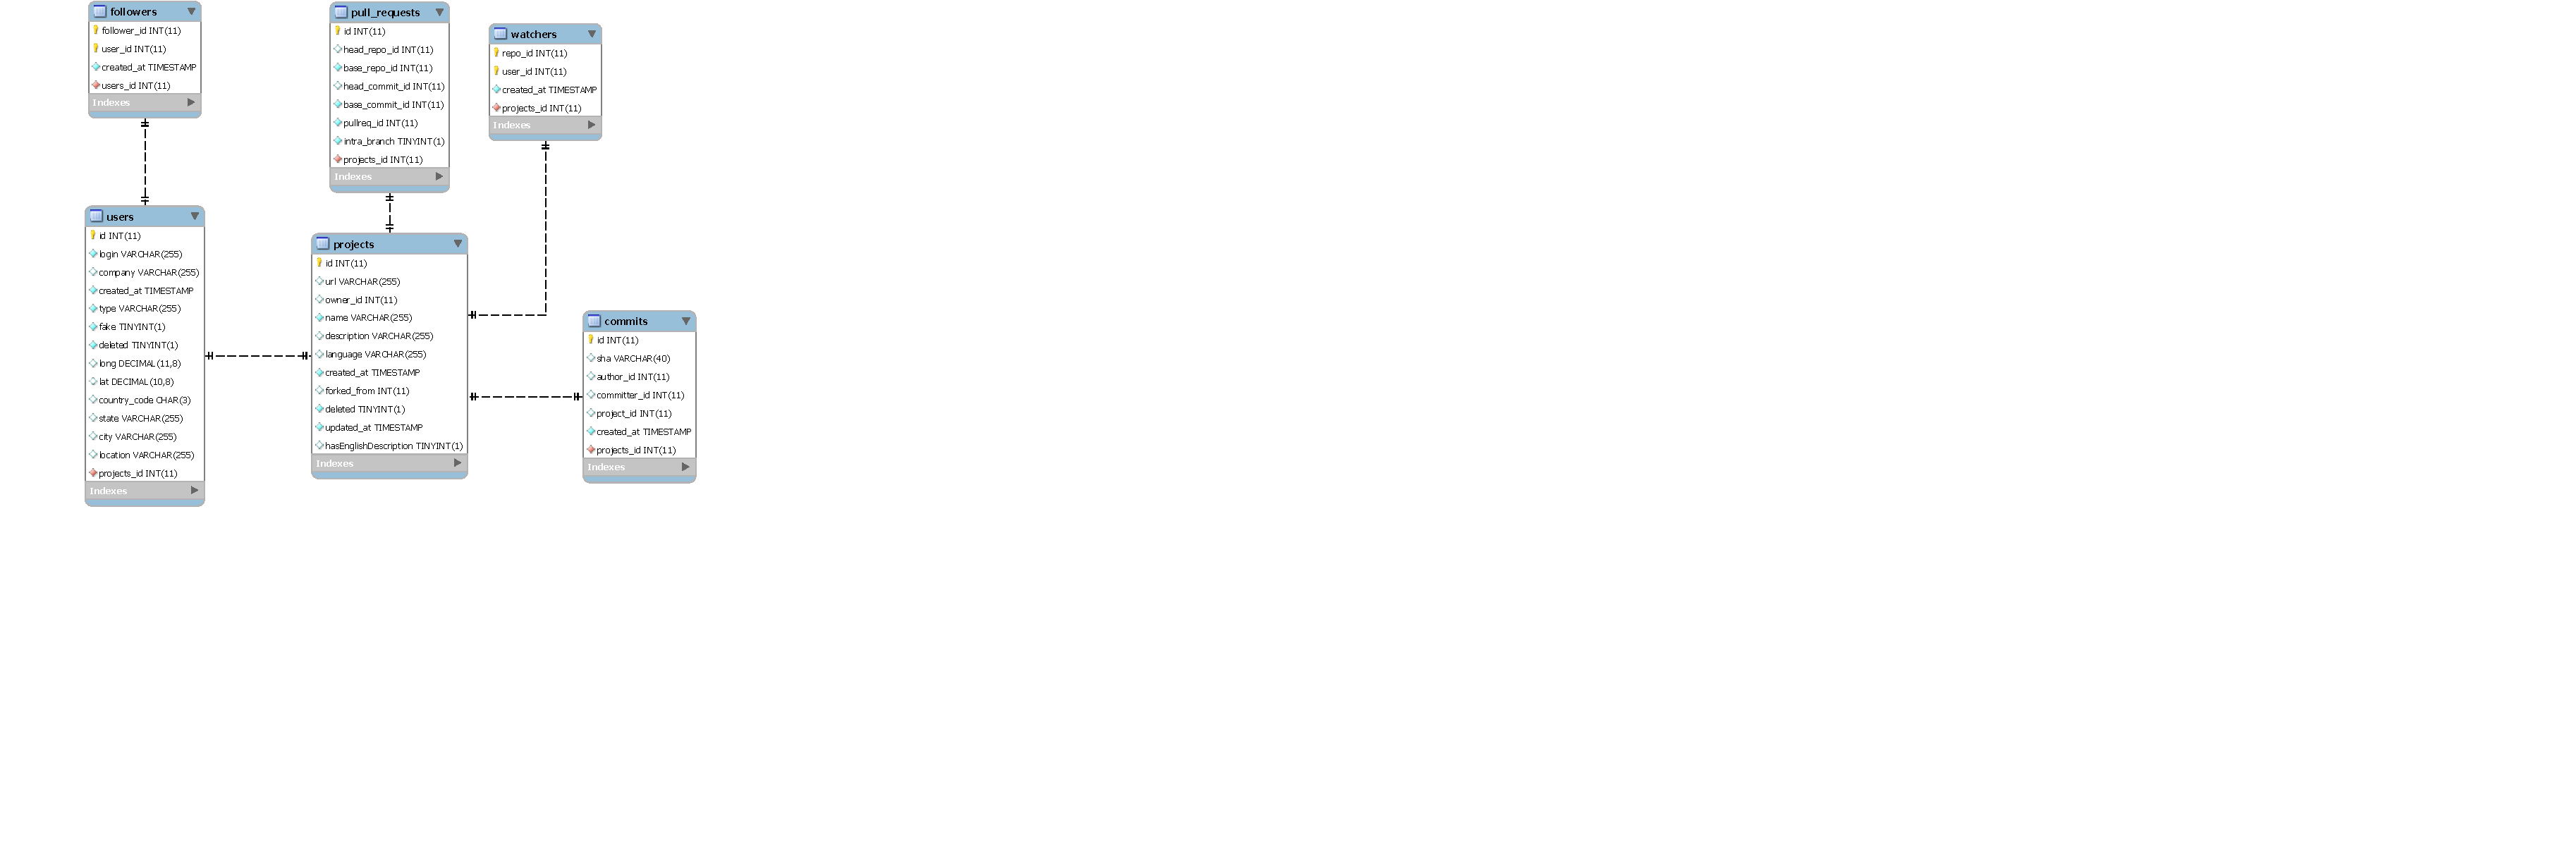
\includegraphics[trim={1cm 7cm 0 0},clip]{capitulo_estudo_caso/tabelas_ghtorrent.pdf} 
  \caption{Tabelas do GHTorrent.}
  \label{fig:tabelas_ghtorrent} 
\end{figure}

Em nosso estudo de caso, os dados fornecidos pelo GHTorrent serão utilizados na seguintes atividades:

\begin{itemize}
\item \textbf{Seleção dos projetos}. A identificação dos projetos do GitHub que foram desenvolvidos em Java. Essa seleção foi realizada utilizando a coluna ``language'' disponibilizada na tabela ``projects'' do GHTorrent.
\item \textbf{Exclusão dos projetos incompatíveis}. Determinar, por meio de heurísticas,  se um repositório é ou não um projeto de software. Um exemplo de heurística aplicada foi excluir projetos que possuem poucos \textit{commits}. De acordo com a literatura, essa é uma das medidas eficientes para evitar a inclusão de repositórios que não são projetos de software. Todas heurísticas utilizadas serão descritas na sessão \ref{secao_cap_estudo_selecao_projetos}.
\item \textbf{Cálculo da colaboração}. Determinar  o volume e a qualidade  da colaboração que um projeto recebeu.
\item \textbf{Cálculo da produtividade}. Alguns dos dados utilizados nos modelos de produtividade serão obtidos por meio do GHTorrent.
\end{itemize}


\subsection{O SonarQube}

Para extrair diversas métricas dos projetos utilizados neste estudo de caso 7.1 da ferramenta SonarQube\cite{campbell2013sonarqube} . Essa ferramenta possibilita verificar diversos aspectos relacionados à qualidade de um projeto de software.  O SonarQube é composto, basicamente, por dois módulos: 

\begin{itemize}

\item \textbf{\textit{Scanner}}: É o responsável por acessar e analisar estaticamente o código-fonte do software.
\item \textbf{Interface web}: Permite a visualização de relatórios a respeito dos dados obtidos pelo \textit{scanner}.

\end{itemize}



Para que o \textit{scanner} possa ser utilizado é necessário que um conjunto de configurações sejam definidas para cada projeto e versão sendo analisada. A Figura \ref{fig:configuracao_sonar_scanner} mostra a função no GitResearch responsável por definir essas configurações. Dentre as configurações necessárias está o identificador único do projeto (\textit{sonar.projectKey}), a versão (\textit{projectVersion}), em qual pasta estão os códigos-fonte (\textit{sonar.sources}), a url da aplicação para internet do SonarQube (\textit{sonar.host.url}) e qual a linguagem utilizada no projeto (\textit{sonar.language}). 


 \begin{figure}[H]
  \centering
  \frame{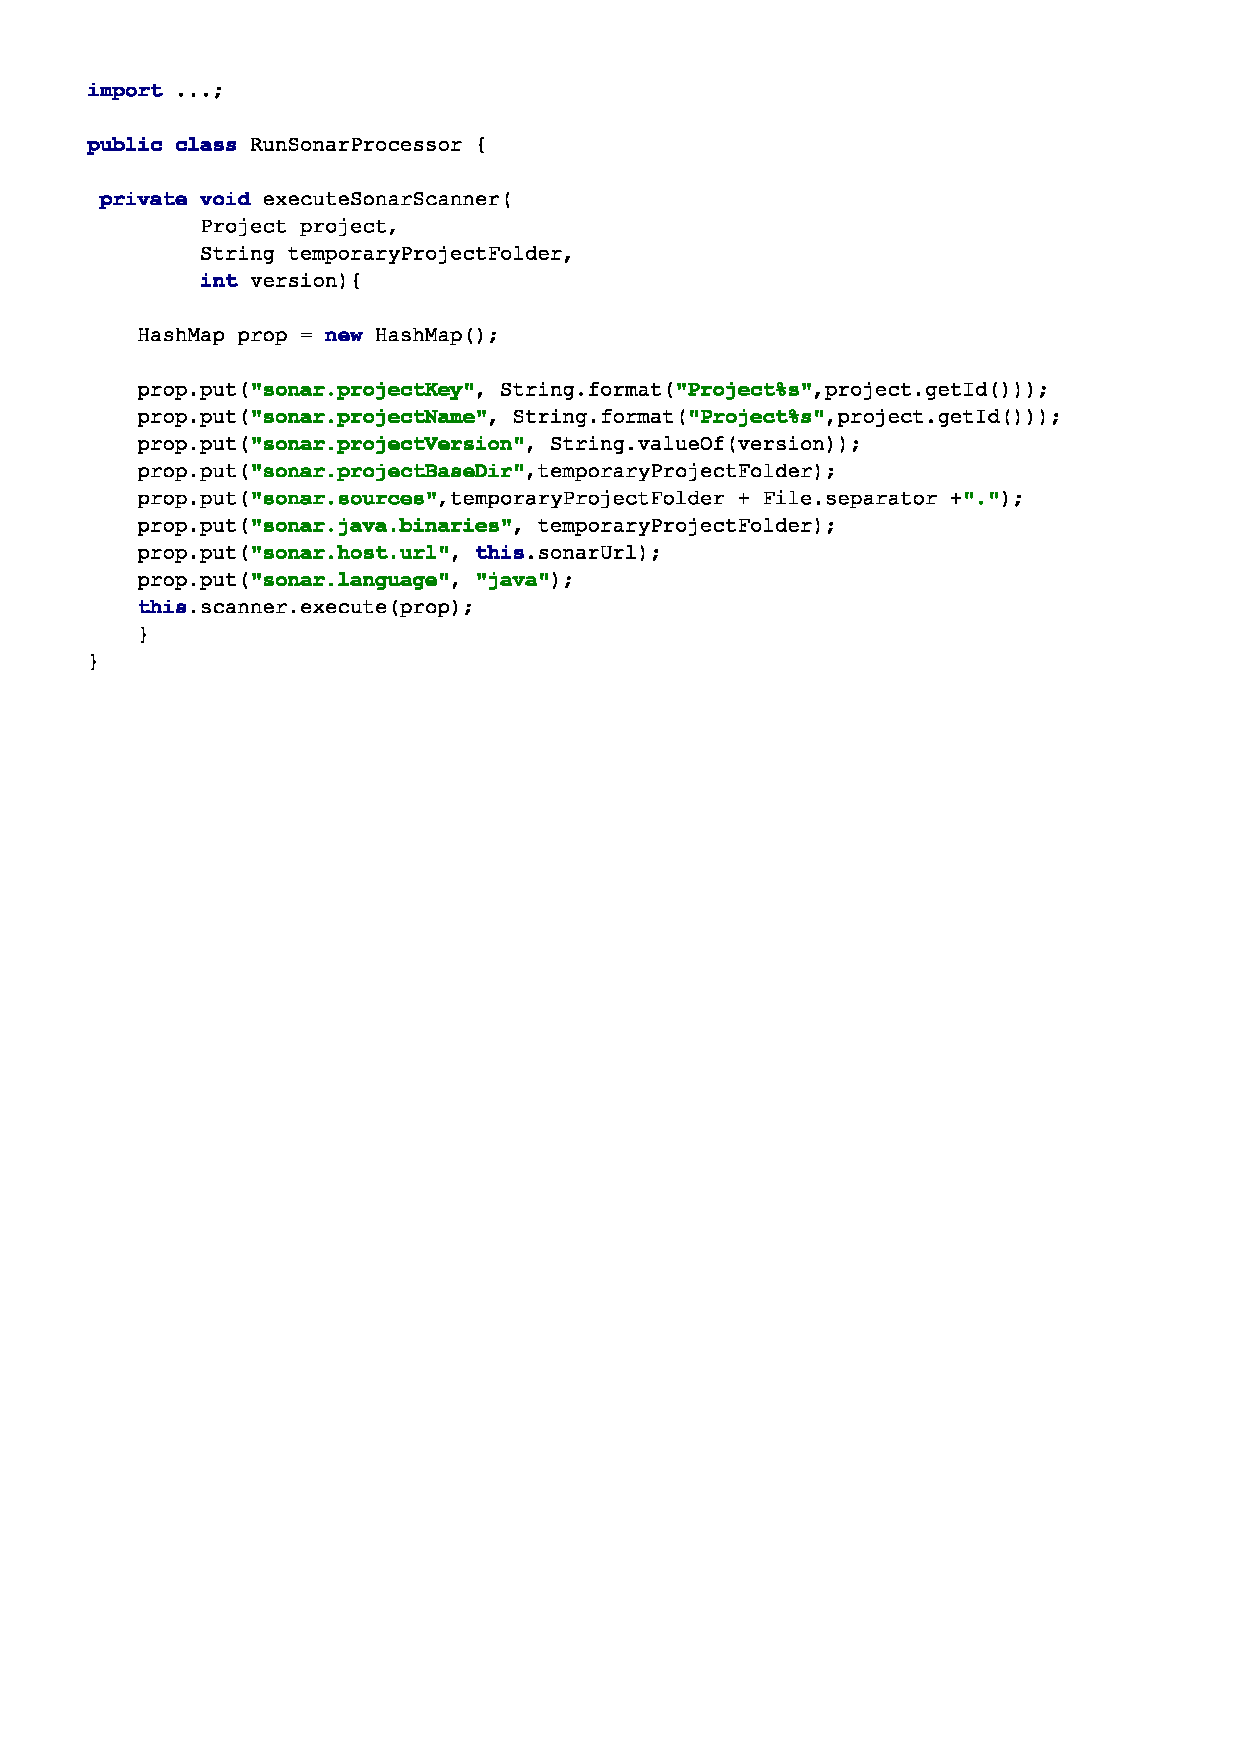
\includegraphics[trim={1cm 18cm 2.5cm 0},clip]{capitulo_estudo_caso/codigo_propriedades_sonar.pdf}} 
  \caption{Código responsável por criar a configuração para a execução do \textit{scanner} do SonarQube no GitResearch.}
  \label{fig:configuracao_sonar_scanner} 
\end{figure}




A Tabela \ref{table:metricas_sonar} contém as métricas que são disponibilizadas pelo SonarQube.  Essas métricas ficam disponíveis no SonarQube automaticamente após a execução do \textit{scanner} em um projeto de software. 

Algumas dessas métricas são calculadas utilizando apenas o código-fonte da aplicação. Esse é o caso, por exemplo, da quantidade de arquivos, linhas de código, funções e classes. Entretanto, algumas das métricas disponibilizadas pelo SonarQube dependem de informações adicionais para serem calculadas. Esse é o caso  da Métrica $VIOLATIONS$. Essa métrica contém a quantidade de violações a regras de qualidade que foram encontradas no código-fonte. Essas regras ficam armazenadas no SonarQube e podem ser alteradas pelo usuário. Neste estudo de caso utilizamos o perfil de regras padrão disponibilizadas pelo SonarQube para a análise de qualidade de projetos java. Esse perfil é chamado de \textit{Sonar Way}\cite{arapidis2012sonar} e é baseado na metodologia de qualidade chamada \textit{sqale}\cite{letouzey2012sqale}.


\def\arraystretch{2.5}
\begin{longtable}{c|c}
\hline
\textbf{Métrica}                                       & \textbf{Descrição} \\ \hline
CODE\_SMELLS              	        &   \pbox{11cm}{Quantidade de trechos do código que contém uma violação a algum princípio fundamental da programação de sistemas\cite{suryanarayana2014refactoring}.}  \\  \hline
COGNITIVE\_COMPLEXITY        &   \pbox{11cm}{Um índice que indica o quão difícil é entender o código-fonte do projeto\cite{campbell2017cognitive}. }  \\ \hline
COMMENT\_LINES                     &  \pbox{11cm}{Quantidade de  linhas de comentários}   \\ \hline
COMMENT\_LINES\_DENSITY    &  \pbox{11cm}{Quantidade de linhas de comentários/(Linhas de código + Quantidade de linhas de comentários) * 100}   \\ \hline
COMPLEXITY                              &  \pbox{11cm}{Complexidade ciclomática do código-fonte\cite{mccabe1976complexity}. }   \\ \hline
DIRECTORIES                            &  \pbox{11cm}{Número de diretórios.}   \\ \hline
DUPLICATED\_LINES                 &  \pbox{11cm}{Linhas duplicadas}   \\ \hline
DUPLICATE\_LINES\_DENSITY  &  \pbox{11cm}{Linhas duplicadas / total de linhas * 100.}   \\ \hline
DUPLICATED\_BLOCKS              &  \pbox{11cm}{Número de blocos de códigos duplicados.}   \\ \hline
DUPLICATED\_FILES                 &  \pbox{11cm}{Número de arquivos duplicados.}   \\ \hline
FILES                                         &  \pbox{11cm}{Número de arquivos.}   \\ \hline
FUNCTIONS                               &  \pbox{11cm}{Número de funções.}   \\ \hline
NLOC                                         &  \pbox{11cm}{Número de linhas que contenham pelo menos um caractere que não seja um espaço, tabulação ou parte de um comentário.}   \\ \hline
SQALE\_DEBT\_RATIO              &  \pbox{11cm}{Razão entre o tempo estimado para resolver a dívida técnica do projeto e o tempo estimado que foi gasto para desenvolver o projeto. }   \\ \hline
SQALE\_RATING                       &  \pbox{11cm}{Uma classificação de 1 até 5 relativa ao nível de dívida técnica do projeto. Projetos com menos dívida técnica recebem a nota 1. }   \\ \hline
STATEMENTS                            &  \pbox{11cm}{Número de declarações no código-fonte.}   \\ \hline
VIOLATIONS                             &  \pbox{11cm}{Número de violações das regras de qualidade definidas no SonarQube.}   \\ \hline

\caption{Métricas extraídas dos projetos.}
\label{table:metricas_sonar}
\end{longtable}
\def\arraystretch{1}




\subsection{Medição da dívida técnica}

Conforme descrevemos no Capítulo \ref{cap:cap2}, existem diversos tipos de dívida técnica. Alguns desses tipos são de difícil medição devido às suas características subjetivas ou contextuais. A dívida técnica de tecnologia, por exemplo, acontece quando um projeto de software está utilizando uma tecnologia obsoleta. Porém, definir se uma tecnologia é ou não obsoleta é uma atividade normalmente subjetiva e sujeita a discordâncias. Já as dívidas técnicas de arquitetura dependem de uma análise contextual para serem medidas.  Esse tipo de dívida é descrito como uma violação a algum princípio ou regra pré-definida a respeito de como deve ocorrer a interação entre os componentes de um software. Contudo, parte dessas regras são específicas para o contexto no qual o software é desenvolvido. Isso acontece seja pelas necessidades do software sendo desenvolvido seja por aspectos relacionados aos desenvolvedores. No caso das dívidas técnicas arquiteturais, existem dificuldades de medição tanto por características contextuais quanto por aspectos subjetivos já que a aderência ou não de uma determinada arquitetura às expectativas de um desenvolvedor é algo subjetivo conforme boa parte dos arcabouços de avaliação de arquiteturas como é o caso do ATAM\cite{kazman2000atam}. Dessa forma, medir certos tipos de dívida técnica é uma tarefa difiícil e em alguns casos inviável de ser feita automaticamente. Por conta disso,  tivemos que limitar os tipos de dívida técnica avaliados neste estudo de caso. Esse recorte foi feito por causa do nosso objetivo de medir quantitativamente e automaticamente o nível de dívida técnica dos projetos. Além disso, essa limitação foi realizada considerando os tipos de dívida técnica que a ferramenta SonarQube consegue medir. Com isso, o nível de dívida técnica que consideraremos em um projeto não será igual ao nível real já que serão considerados apenas alguns tipos de dívida.

A medição da dívida técnica é feita pelo SonarQube usando as regras definidas no perfil de qualidade utilizado no projeto. O nível de dívida técnica de um projeto é equivalente à soma do tempo estimado para alterar seu código-fonte de forma que todas as violações a regras de qualidade fossem eliminadas. O SonarQube calcula o nível de dívida técnica de um projeto seguindo os seguintes passos:

\begin{enumerate}
\item Escaneia o código-fonte do software em busca de violações às regras contidas no perfil de qualidade utilizado. Em nosso caso, utilizamos o perfil padrão chamado  \textit{Sonar Way}\cite{arapidis2012sonar}.
\item A cada violação encontrada, é adicionada uma quantidade de tempo ao tempo total necessário para eliminar todas as dívidas técnicas do projeto.
\item O nível de dívida técnica de um projeto é então calculado pela razão entre o tempo total estimado para desenvolver o software  e o tempo total que seria gasto para eliminar todas as dívidas técnicas. Esse cálculo é armazenado na métrica SQALE\_DEBT\_RATIO conforme mostrado na Tabela \ref{table:metricas_sonar}
\end{enumerate}

 A Tabela \ref{table:regras_sonar_way} apresenta algumas das regras de qualidade definidas no perfil padrão do SonarQube para a análise de projetos Java(\textit{Sonar Way}) e a quantidade de minutos estimados para eliminar cada uma das ocorrências de violações de cada regra.  

Forneceremos um exemplo de cálculo da dívida técnica utilizando o SonarQube. Para isso, analisaremos 2 projetos conforme a Tabela \ref{td_ratio_example}. O primeiro projeto tem 45.600 minutos de dívida técnica. Isso significa que após o SonarQube analisar todo o projeto, ele encontrou uma quantidade de dívidas que, somadas, levariam 45.600 minutos para serem resolvidas. Além disso, o  primeiro projeto possui  80.000 linhas de código-fonte. Com isso, o nível de dívida técnica do projeto 1 é calculado como $\frac{45.600}{80.000*m}$ sendo $m$ a quantidade de tempo que se estima necessária para escrever uma linha de código. O SonarQube usa como padrão 30 minutos para a variável $m$. No caso do projeto 1, o nível de dívida técnica foi calculado como 1,9\%. Isso significa que seriam gastos para eliminar a dívida técnica desse projeto 1,9\% do esforço necessário para construir o projeto inteiro. De acordo com Jesus et al. \cite{de2017technical}, um índice abaixo de 3\% é considerado baixo; logo, o projeto 1 tem um nível baixo de dívida técnica.  Já o projeto 2, conforme a Tabela \ref{td_ratio_example} possui a mesma quantidade de dívida técnica medida em minutos. Entretanto, medido em número de linhas de código, o projeto 2 é muito menor do que o projeto 1. Isso fez com que o nível de dívida técnica do projeto 2 fosse calcado como 11,7\%, ou seja, muito maior do que o projeto 1. Com isso, mesmo tendo o mesmo volume de dívida técnica que o projeto 1, de acordo com a estratégia de medição adotada, o projeto 2 é considerado pior do que o projeto 1 em termos de dívida técnica. Isso acontece porque o SonarQube
calcula o nível de dívida técnica de um projeto de uma forma proporcional ao seu tamanho.


\begin{table}[H]
\centering


\def\arraystretch{2.5}%
%\normalsize
\begin{tabular}{ccccc}
\hline
        \textbf{Projeto}   & \textbf{Dívida técnica em minutos}  &  \textbf{Linhas de código} & \textbf{Cálculo} & \textbf{\textit{Debt Ratio}}\\ \hline
1 & 45600               & 80000         & $\frac{45600}{80000*m} $ &  1,9 \%    \\ \hline
2 & 45600               & 13000         & $\frac{45600}{80000*m} $ &  11,7  \%   \\ \hline
\end{tabular}
\caption{Exemplo de cálculo da dívida técnica com o SonarQube. A variável \textit{m} representa o tempo necessário para escrever uma linha de código. O valor padrão no SonarQube é de 30 minutos. Adaptado de \cite{de2017technical}.}
\end{table}
\label{td_ratio_example}


\begin{table}[H]

\normalsize
\centering
\def\arraystretch{2.5}%
\begin{tabular}{|c|c|c|}

\hline
\textbf{Categoria}  & \textbf{Descrição} & \textbf{Minutos}  \\ \hline
Mutabilidade           &  \pbox{10cm}{Bloco de código duplicado.} & \pbox{1cm}{ 60 }  \\ \hline
Manutenção         &  \pbox{10cm}{Variável não usada.} & \pbox{1cm}{ 10 }  \\ \hline
Testabilidade           &   \pbox{10cm}{Complexidade ciclomática \cite{mccabe1976complexity} maior do que 10.} & \pbox{1cm}{ 11  }  \\ \hline
Reusabilidade        &   \pbox{10cm}{ Parâmetro usado como seleção em um método público. } & \pbox{1cm}{ 15  }  \\ \hline
Confiabilidade         &   \pbox{10cm}{A condição de um laço nunca será verdadeira.} & \pbox{1cm}{ 10  }  \\ \hline
Segurança                &   \pbox{10cm}{Comandos sendo enviados para o sistema operacional sem nenhuma validação } & \pbox{1cm}{ 30  }  \\ \hline
Portabilidade         &  \pbox{10cm}{Uso de métodos descontinuados.} & \pbox{1cm}{ 15  }  \\ \hline
Manutenção         &  \pbox{10cm}{Existência de código-fonte comentado.} & \pbox{1cm}{ 5 }  \\ \hline


\end{tabular}

\caption{Exemplos de regras para identificação de dívidas técnicas no SonarQube.}

\end{table}
\label{table:regras_sonar_way}
\def\arraystretch{1}%





\subsection{Limitações na medição da dívida técnica}


É possível identificar algumas limitações em relação à forma como o SonarQube realiza a medição do nível de dívida técnica de um projeto. A primeira delas é a falta de uma verificação empírica para a quantidade de minutos necessários para corrigir cada dívida. Por exemplo, de acordo com a Tabela \ref{table:regras_sonar_way}, remover um bloco de código duplicado levaria 60 minutos. Porém, não é possível encontrar na documentação da ferramenta nenhuma indicação de como esse valor foi definido. Com isso o tempo médio para refatorar o código-fonte e resolver esse problema pode ser muito maior ou muito menor do que 60 minutos. Outro ponto questionável é a lista de regras que são usadas para identificar dívidas técnicas na configuração padrão do SonarQube. Não há também na documentação da ferramenta qualquer menção a qual metodologia foi utilizada para criar essa lista. Inclusive, a capacidade de identificar dívidas técnicas por meio de algumas das regras utilizadas são claramente questionáveis. 

Apesar das limitações, o SonarQube tem sido usado efetivamente para a análise da dívida técnica em projetos de software, inclusive no contexto de pesquisas científicas. Uma das evidências da eficácia dessa ferramenta foi obtida por Marek et al.\cite{stochel2012value}. Nesse trabalho os autores realizaram um \textit{survey} com especialistas para que eles analisassem e indicassem o nível de dívida técnica de alguns projetos. Os dados obtidos foram então comparados com a medição realizada pelo SonarQube. As diferenças entre os dois resultados foram muito pequenas. Isso trouxe evidências de que a dívida técnica medida pelo SonarQube é tão precisa quanto aquela medida por especialistas.  Além disso, uma pesquisa realizada por Fontana et al.\cite{fontana2016tool} comparou algumas ferramentas que são capazes de calcular a dívida técnica de um projeto. Os autores chegaram à conclusão de que o SonarQube é a ferramenta mais precisa atualmente disponível. Apesar disso, conforme apontado por Fonta et al.\cite{fontana2016technical}, o índice de dívida técnica calculado pelo SonarQube não é apropriado para a análise individual de projetos. Em vez disso, esse índice deve ser usado apenas para comparar projetos diferentes.  


\section{Conclusões}

Neste capítulo apresentamos o planejamento para o estudo de caso que realizamos nesta pesquisa. Inicialmente, introduzimos as cinco etapas desse estudo de caso: seleção, agrupamento, extração, cálculo das métricas e análise dos dados. Foram fornecidos alguns detalhes a respeito das atividades dentro de cada uma dessas etapas e como elas serão executadas. Depois, apresentamos a ferramenta GitResearch. Essa ferramenta será utilizada para automatizar grande parte das atividades realizadas no estudo de caso. Por fim, apresentamos as outras plataformas e ferramentas existentes que foram utilizadas: Github, GHTorrent e SonarQube. 










